\documentclass[a4paper,parskip]{scrartcl}

\usepackage{lmodern}
\renewcommand*\familydefault{\sfdefault}
\usepackage[T1]{fontenc}

\usepackage[ngerman]{babel} %german english spell checking
\usepackage[utf8]{inputenc} %allows ä,ö,ü and others
\usepackage{multicol} %allows multiple columns
\usepackage{enumitem} %allows to change enumerate style
\usepackage[colorlinks=true,pdfborder={0 0 0},urlcolor=cyan,linkcolor=black]{hyperref} %allows links
\usepackage{verbatim} %allows code
\usepackage{graphicx} %allows images
\usepackage{amssymb} %allows symbols for number sets

\setlist{nosep} %smaller lists, less space between lines

\title{Dokumentation - MindMap}
\author{Lorenz Rasch \& Dominik Meister}

\begin{document}
\maketitle
\tableofcontents
\pagebreak
\section{Vision}
Ein Mind-Map erlaubt es Themen in ihrer ganzen breite einfach und verständlich darzustellen. Oft wird dies auf Papier während eines Meetings oder bei der Planung gemacht.\\
Mit unserer Software wollen wir das Konzept von den Grenzen des Papiers befreien.\\
Ein Mind-Map soll einfach zu erstellen und verändern sein. Ausserdem soll es gespeichert und gedruckt werden können.

\section{Evaluation}
\subsection{Use Cases \& User Stories}
\subsection{Anforderungen}

\section{Design}
\subsection{Systemkontext}
\subsection{System Sequence Diagram}
\subsection{Domainmodel}
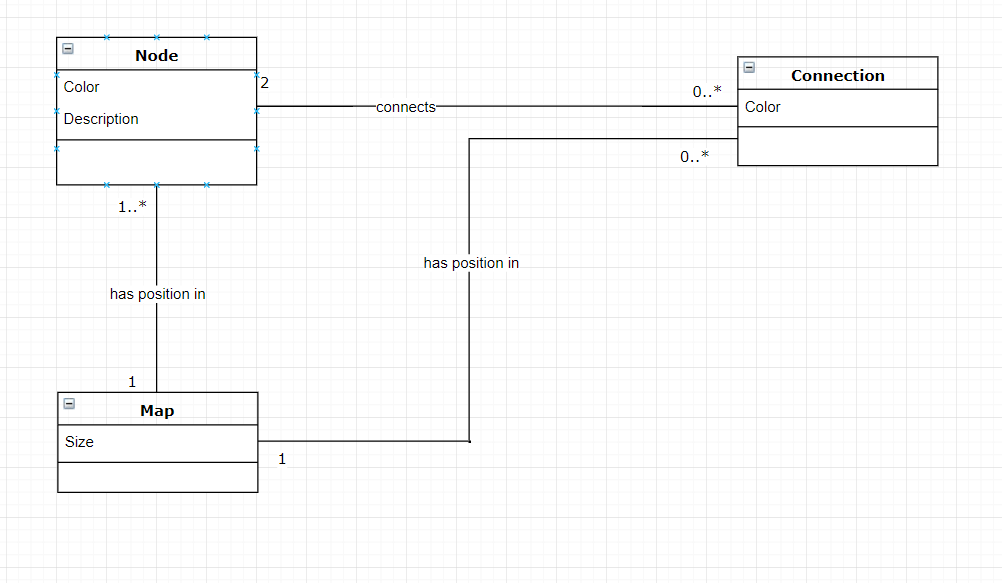
\includegraphics[width=\linewidth]{DomainModel.PNG}
\subsection{UML Diagramme}

\section{Entwicklung}
\subsection{Sprint 1}
\subsection{Sprint 2}
\subsection{Sprint 3}
\subsection{Sprint 4}

\section{Test}

\section{Glossar}

\end{document}